\chapter{科技文档}

\begin{quote}
    智慧人积存知识,愚妄人的口速致败坏。
    
    \hfill《圣经·箴言》10:14
\end{quote}

现在,终于到了跟你聊聊所谓\emph{科技}文档特性的时刻。虽然关于数学式和其他方程的问题已经在第3章妥善解决,但还有一块骨头要啃:参考文献。对于这个问题,虽然不能一口吃个胖子,但接下来的内容可以让你大幅简化工作。在本章,我们还会解释生成索引的机制。

本章首先会介绍起草文章的几点特别之处,然后展示参考文献的生成和索引的生成,最后介绍将大篇幅文档拆解成几个小部分的实用方法。

\section{文章(article)}

为了起草一篇文章,没有什么新内容可以介绍的,我们目前为止见过的所有内容都适用。只需要注意,在文前部分中,可以使用以下指令:

\begin{itemize}
    \item \verb|\title|,定义标题;
    \item \verb|\date|,定义日期;
    \item \verb|\author|,定义作者团队;
    \item \verb|\thanks|,定义作者单位。
\end{itemize}

若要利用这些定义来插入标题,需要在\verb|\begin{document}|之\textbf{后}插入指令\verb|\maketitle|:

\begin{dmd}
\begin{verbatim}
\documentclass{article}
\title{Le seuillage à 128 : une révolution !}
\author{M. C. Orlanrien\\
        Institut du Pixel\\
        42007 Saint-Etienne---FRANCE}
\date{2 Avril 1927}
\begin{document}
\end{verbatim}
\backslash maketitle\textsl{\% 标题插到此处}\\
...\\
\verb|\end{document}|
\end{dmd}

此处重复一遍\jz{
    因为传授知识就是重复的过程。
}:标题是由指令\verb|\maketitle|生成并插入的,而不是文前部分的定义。

通常来说,会议或期刊提供的模板文件中会引入一些变化(例如使用\verb|\address|分隔作者和其地址),但基本原理是一致的。

\section{参考文献}

由两种方式可以使用\LaTeX 起草文章的参考文献部分。其中,可以称得上是“手动”的方式是,在文章中插入环境\dm{thebibliography}。另一种方式,即此处要介绍的方式,是使用\bib ,主要分为如下步骤。

\begin{enumerate}
    \item 创建一个或多个参数文件,包含\bib 格式的各条参考文献入口(entrée;文章、会议……)。这个步骤不可避免地需要我们去\emph{输入}。
    \item 在文档中,使用指令\verb|\cite|去引用这些入口。
    \item 参考文献会自动根据你选择的特殊风格排版。
\end{enumerate}

这种方法的优势是,对于每条参考文献,你只需输入一次。此外,考虑到可以使用\emph{风格文件},你不用去担心它的版式。有几十种风格文件,对应各种标准,包含期刊和其他会议所使用的标准。我们也可以在互联网上找到\bib 格式的参考文献数据库,可以在文档中直接使用。

我们重复一遍:参考文献有多种标准。但不幸的是,一些期刊偏偏喜欢指定属于自己的参考文献格式。有朝一日你在这种期刊上发表文章时,就需要去创建或调整风格文件。为了实现这一点,可以去查找工具\textsf{makebst}。

\subsection{\dm{.bib}文件}

第一个操作是构建\jz{
    \textbf{Emacs}的Auc\TeX 组件包含了很好用的\bib 模式。
}参考文献文件,其扩展名最好为\dm{.bib}。该文件需要遵循特殊的语法。首先需要知道,\bib 通过\emph{类型(type)}区分每个入口。这样一来,每个入口都带有一个文档类型:图书、文章、会议、科技报告……一共有二十多种不用的文档类型。

\begin{ii}
正常来说,我们可以在伴随\LaTeX 发行版提供的文件找到名为\bib ing的文件(命名为\dm{btxdoc.pdf}),由奥兰·帕塔什尼克(Oran Patashnik)在约二十年前创作。该文件包含有关构建\bib 格式文件方法的重要信息来源。
\end{ii}

每个入口\emph{类型}都包含一定数量描述该入口的\emph{字段(champ)}。参考文件入口的结构如下:

\begin{dmd}
@\codereplace{入口}\{\codereplace{关键描述},\\
\verb|  |\codereplace{字段$_1$}\ =\ \{...\},\\
\verb|  |\codereplace{字段$_2$}\ =\ \{...\},\\
\verb|  |...\\
\verb|  |\codereplace{字段$_n$}\ =\ \{...\},\\
\}
\end{dmd}

其中,\codereplace{入口}表示文档类型(\dm{article}、\dm{inproceedings}等),\codereplace{字段$_1$}、\codereplace{字段$_2$}……\codereplace{字段$_n$}表示参考文献入口的不同字段。这些\bib 的保留字可以以大写或小写形式输入。

符号\codereplace{关键描述}需要以唯一方法描述该文档,以备通过用于识别标签的符号\verb|\label|来重新找到。为了你能够快速上手\bib ,接下来的示例综合了三个你需要使用的基本入口。

\subsubsection{期刊文章}

有一篇期刊文章需要以如下形式输入:

\begin{dmd}
\begin{verbatim}
@article{qtz:UchArb,
    author ={Uchiyama, Toshio and Arbib, Michael A.},
    title = {Color Image Segmentation
            Using Competitive Learning},
    journal=pami,
    volume =16, number=2, pages={1197--1206},
    month=dec, year=1994}
\end{verbatim}
\end{dmd}

有以下几点需要注意。

\begin{enumerate}
    \item 字段\dm{author}、\dm{title}、\dm{journal}、\dm{year}是必需的。
    \item 对于作者\jz{
        此处关于作者的注意事项对于其他入口(会议、书等)也同样适用。
    }姓名,需要遵循\codereplace{姓}、\codereplace{名}的顺序。\textbf{所有}作者姓名都需要以\dm{and}分隔。
    \item 对于复合姓或其他特殊作者名,可以以如下形式输入:
    \begin{center}
        \dm{author="de la Motte Beuvron, Alain"}
    \end{center}
    其中遵循的顺序为:\codereplace{特殊组成部分}、\codereplace{姓}、\codereplace{名}。逗号作为分割符,起到与上例中相似的作用。
    \item 所有月份可以以字符串的形式给出,如\dm{jan}、\dm{feb}、\dm{mar}等。
\end{enumerate}


在\dm{.bib}文件的开头,为简洁起见,我们已经创建了\emph{缩写}\dm{pami}:

\begin{dmd}
\begin{verbatim}
@string{pami="IEEE transactions on Pattern Analysis and
              Machine Intelligence"}
\end{verbatim}
\end{dmd}

\subsubsection{会议析出文章}

没错,\bib 会区分对待\emph{期刊}和\emph{会议}中的文章。格式结构与上例很相似,只不过\dm{booktitle}用于会议标题而不是期刊标题:

\begin{dmd}
\begin{verbatim}
@Inproceedings{qtz:BouOrch,
    author={Bouman, Charles A. and Orchard, Michael T.}
    title={Color Image Display with a Limited Palette Size},
    booktitle={SPIE Conference on Visual Communications
               and Image Processing},
    volume=1199,pages={522--533},
    year=1989}
\end{verbatim}
\end{dmd}

这里,\dm{author}、\dm{title}、\dm{booktitle}、\dm{year}是必填字段,我们可以选用\dm{volume}和\dm{number}。

\subsubsection{图书片段}

相比于整本书,我们经常指参考其中的一个片段——若干章、若干页:

\begin{dmd}
\begin{verbatim}
@inBook{col:McA,
    author =    {MacAdam, David L.},
    title =     {Color Measurement},
    chapter =   4,
    pages   =   {48--49},
    publisher = {Springer-Verlag},
    year =      1985}
\end{verbatim}
\end{dmd}

强制字段为:\dm{author}、\dm{title}、\dm{chapter}或\dm{pages}、\dm{publisher} (出版方),以及\dm{year}。

\begin{ii}
我们再次强烈建议你使用Emacs组件Auc\TeX 的\bib 模式。特别是该模式为你提供了包含所有入口类型的菜单。选择菜单中的一项,就可以在你的文件中插入入口“骨架”。该组件可以在\wz{ftp.lip6.fr/pub/TeX/CTAN/support/auctex}下载,也可以以包Debian的形式获取。
\end{ii}

\subsection{参考文献的标注}

一旦参考文献建立完成,就可以即刻在文档中借助关键描述使用指令\verb|\cite|来标明引用:

\begin{dmd}
\backslash cite\{\codereplace{关键描述}\}
\end{dmd}

指令\verb|\cite|有如下功能:

\begin{enumerate}
    \item 根据选择的风格插入跳转符号(如[2]、[Loz95]等);
    \item 在文档的参考文献部分中添加所引用的文章。
\end{enumerate}

\begin{ii}
    文章(此处指广义的文章)只有在被\verb|cite|作为引用对象时才会出现在参考文献中。若要列出未于正文中直接引用的文章,则需要使用指令\verb|\nocite{|\codereplace{关键描述}\verb|}|将\codereplace{关键描述}的对应文章插入文档的参考文献部分。此外,指令\verb|\nocite{*}|会将\dm{.bib}文件中的\emph{所有}入口插入文档。
\end{ii}

在实际进入生成参考文献的步骤前,需要在\LaTeX 文档末尾添加对以下指令的引用来指定参考文献的风格:

\begin{dmd}
\verb|\bibliographystyle|
\end{dmd}

然后,引用如下指令来实际插入参考文献:

\begin{dmd}
\verb|\bibliography|
\end{dmd}

对于风格,有:

\begin{dmd}
\backslash bibliographystyle\{\codereplace{风格}\}
\end{dmd}

\LaTeX 预定义的风格\jz{
    在CTAN网站的\dm{biblio/bibtex/contrib}可以找到几十种可供使用的其他风格。
}如下。

\begin{itemize}
    \item \dm{plain},引用的形式为[2],参考文献会根据作者名排序。
    \item \dm{unsrt},参考文献根据引用顺序排序。会议文章经常使用这种风格。
    \item \dm{alphs},引用的形式为“作者缩写+年份”。
\end{itemize}

接下来,需要指定哪些文件包含了文档中指令\verb|\cite|所“指向”的那些参考文献:

\begin{dmd}
\backslash bibliography\{\codereplace{文件$_1$}, \codereplace{文件$_2$}, \codereplace{……}\}
\end{dmd}

这样的指令会使\bib 在处理过程中包含\codereplace{文件$_1$}\dm{.bib}、\codereplace{文件$_2$}\dm{.bib}……

\subsection{生成参考文献}

生成参考文献的步骤如下。

\begin{enumerate}
    \item 借助\LaTeX 实现第一次编译,使得辅助文件\dm{doc.aux}包含\emph{引用标注}信息:
    
    \begin{center}
        \includegraphics{img/bibtex1}
    \end{center}
    
    \item 运行\bib ,在文件\dm{doc.bbl}中生成参考文献:
    
    \dmh{bibtex doc}

    \begin{center}
        \includegraphics{img/bibtex2}
    \end{center}

    \item 借助\LaTeX 的第二次编译插入参考文献:
    
    \begin{center}
        \includegraphics{img/bibtex3}
    \end{center}

    %TODO 图片中bibtex和latex替换

    \item 通过第三次编译解析交叉引用。
\end{enumerate}

如果你对这个过程感到好奇,可以看到:文件\dm{doc.bbl}包含了环境\dm{thebibliography}以供随时使用\jz{
    也就是说,你如果不使用\bib ,就必须着手处理该环境。
};文件\dm{doc.blg}是与那些\dm{.log}文件相似的“日志”文件,储存着上一次使用\bib 时一些可能出现的错误或警告。

\begin{exclamation}
程序\bib 对环境\dm{BIBINPUTS}中的参数敏感。因此,在某些情况下,有必要在\linebreak\dm{.bash\_profile}中添加以下一行命令:

\dmh{export BIBINPUTS=\$HOME/LaTeX/biblio//:}

这样可以使\bib 在目录\dm{\$HOME/LaTeX/biblio}中搜索你的参考文献文件(此处的目录为示例)。
\end{exclamation}

\section{索引}

生成索引需要依靠以下两个概念:

\begin{enumerate}
    \item 在\LaTeX 文档中添加指令\verb|\index|来添加索引入口;
    \item 使用程序\textbf{makeindex}来正确地抽取和展示索引。
\end{enumerate}

负责在文档中插入索引部分的是指令\verb|\printindex|。可以将该指令与\verb|\tableofcontents|类比。

\subsection{必要步骤}

这里给出简短的索引制作备忘录:

\begin{enumerate}
    \item 在主文件中插入两条指令:
    \begin{dmd}
    \begin{tabbing}
12345678902234567890\=\kill
\verb|\makeindex|\>\textsf{$\leftarrow$告知\LaTeX 需要生成索引}\\
\verb|\begin{document}|\\
{\rmfamily ……文档正文……}\\
\verb|\printindex|\>\textsf{$\leftarrow$在文档中实际插入索引部分}\\
\verb|\end{document}|
    \end{tabbing}
    \end{dmd}

    \item 插入索引入口:
\begin{dmd}
\begin{tabbing}
12345678902234567890\=\kill
\verb|\index{bidule}|\>\textsf{$\leftarrow$在索引中插入“bidule”}
\end{tabbing}
\end{dmd}

    \item 为了为文档\dm{doc.tex}生成索引,需要成功执行以下三条指令:
    
    \begin{dmd}
        latex doc\\makeindex doc\\latex doc
    \end{dmd}
\end{enumerate}

\subsection{机制细节}

文档\dm{doc.tex}的第一次编译(在满足文前部分带有控制序列\verb|\makeindex|的条件下)会生成包含“散装”的索引入口文件\dm{doc.idx}:

\begin{center}
    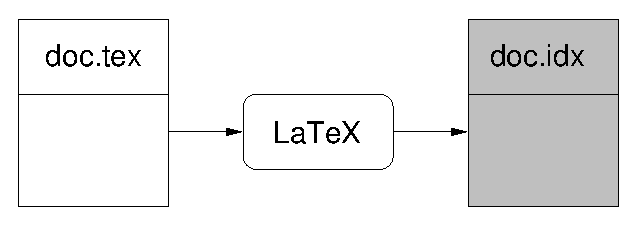
\includegraphics{img/makeindex1}
\end{center}

接下来,使用\textsf{makeindex},在这个文件\dm{doc.idx}中整理条目、删除重复项,并将结果存入\dm{doc.ind}。执行轨迹会存储在\dm{doc.ilg}中:

\begin{center}
    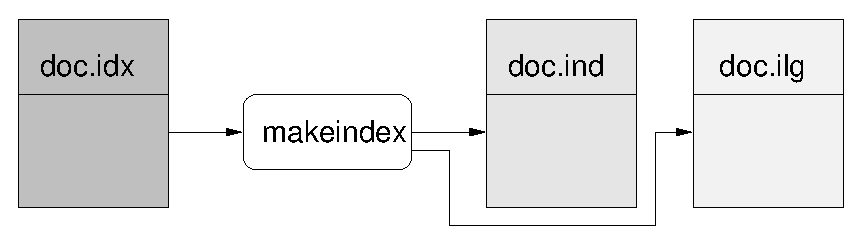
\includegraphics{img/makeindex2}
\end{center}

终端下运行的\textsf{makeindex}嘴很碎。如下展示了它生成文档索引时展示的信息:

\begin{dmd}
\begin{verbatim}
This is makeindex, version 2.13 [07-Mar-1997] (using kpathsea).
Scanning input file guide.idx....done (982 entries accepted, 0 rejected).
Sorting entries...........done (11254 comparisons).
Generating output file guide.ind....done (745 lines written, 0 warnings).
Output written in guide.ind.
Transcript written in guide.ilg.
\end{verbatim}
\end{dmd}

因此,在运行失败的情况下,需要警惕可能出现的抛出和警告(\emph{warning})。\LaTeX 的第二次编译可以在\dm{doc.tex}中指令\verb|\printindex|指出的位置插入格式化过的索引(文件\dm{doc.ind}):

\begin{center}
    \includegraphics{img/makeindex3}
\end{center}

\begin{ii}
工具makeindex可以识别选项\dm{-s},该选项用于为索引指定\emph{风格}。这里所说的风格定义在带有扩展名\dm{.ist}的文件中,可以改变索引的排版央视。可以以如下方式修改文件风格:

\dmh{makeindex -s}\codereplace{文件风格}\codereplace{主文件}

可以在你使用的发行版中寻找风格文件并测试它们。
\end{ii}

\subsection{索引入口的不同类型}

目前为止,我们看到的索引形式都是\emph{\codereplace{索引词}及\codereplace{页码}},但也可以使用更讲究些的入口形式,至少包含如下三种。

\begin{enumerate}
    \item 带有层级的入口:
    
    \begin{dmd}
    \verb|\index{bidule!chouette}|
    \end{dmd}

    该指令可以在索引中插入“bidule”的子入口“bidule”。

    \item 跨页入口:
\begin{dmd}
\begin{tabbing}
12345678902234567890\=\kill
\verb+\index{bidule|(}+\>\textsf{$\leftarrow$位于第$i$页}\\
\verb+\index{bidule|)}+\>\textsf{$\leftarrow$位于第$j$页}
\end{tabbing}
\end{dmd}
    该指令插入的索引形式为bidule $i$--$j$。

    \item 符号化的入口:
    
    \begin{dmd}
    \verb|\index{alpha@\alpha}|
    \end{dmd}

    这样的指令会在索引中插入$\alpha$,并按“alpha”将其分类。同样地,以下指令会在索引中插入“épluche”,但分类时会将首字母看作“e”:

    \begin{dmd}
    \verb|\index{eplucher@éplucher}|
    \end{dmd}
\end{enumerate}

此处列出的最后一个格式同样可以用于为索引插入带有特殊版式的入口。例如:

\begin{dmd}
\verb|\index{bonjour@\textbf{bonjour}}|
\end{dmd}

该指令可以在索引中插入\textbf{bonjour}(即将bonjour加粗),同时按“bonjour”将该入口分类。此外,借助以下指令,我们还可以以特殊版式显示页码:

\begin{dmd}
\backslash index\{\codereplace{入口}|\codereplace{版式指令}\}
\end{dmd}

例如:

\begin{dmd}
\verb+\index{bidule|textbf}+
\end{dmd}

该指令可以让索引中“bidule”的页码显示为加粗样式(注意,在版式指令中没有符号\verb|\|)。

\subsection{术语词典}

有时,我们需要详细列出文档中一些术语的含义。文档中重新组织这些术语解释的部分称为\emph{术语词典(glossaire)}。为了生成术语词典,需要采用与生成\celan{\S 6.3.1}索引相似的方法,只需做一些小的改动,将在11.6节详细介绍。

\section{拆分文档}

如果文档的篇幅很长,我们可以将其自然地按章或部分来拆解。因此,建议创建一个\emph{主}文档,并在其中包含各章或各部分。主文档的形式如下:

\begin{dmd}
\begin{verbatim}
\documentclass{book}

\begin{document}
\end{verbatim}
\verb+\frontmatter +\textsl{\% 所有介绍性的文字}
\begin{verbatim}
\include{preface}
\tableofcontents
\end{verbatim}
\verb+\mainmatter +\textsl{\% 文档的“主体”}
\begin{verbatim}
\part{关于\LaTeX 的那些你想知道却从不敢问的问题}

\chapter{基本原则}

人若身患漏症,他因这漏症就不洁净了。——《圣经·利未记》15:2

本章介绍\LaTeX 的基本原理。你将会看到关于\LaTeX 安装的简介、使用\LaTeX 的基本“流程”(session)介绍、文章格式的结构、使用变音符号的注意事项,认识几个工具,以及了解面对编译错误消息时的态度。

\section{安装}

你想安装\LaTeX 吗?你将要安装的是\LaTeX 的其中一个\textit{发行版},具体的版本取决于你的操作系统\jz{
    如果你不知道操作系统是什么东西,那么你使用的是macOS;如果你不知道你的计算机用的\textit{具体是哪个}操作系统,那么你在用Windows;否则,你在用UNIX……
}。发行版中带有可以自动安装和配置\LaTeX 、\TeX 和其他相关内容的程序。

\paragraph*{对于UNIX}我们可以找到称为te\TeX 的发行版,虽然它的开发早在2006年就停止了。今天,我们一般安装\TeX Live(\wz{http://www.tug.org/texlive})。

\paragraph*{对于macOS}建议安装的发行版是Mac\TeX(\wz{http://www.tug.org/mactex})。

\paragraph*{对于Windows}最简单的方式无疑是选择pro\TeX t(\wz{http://www.tug.org/protext})。它会安装称为MiK\TeX 的发行版(\wz{http://www.miktex.org})和几个开发工具,其中包含一个查看PostScript文件的程序(\textsf{gsview})。

偶尔,需要在为发行版中搭配一款文字编辑器(如果其中没有包含),因为你很快就能看到,使用\LaTeX 就是在文件中输入文字和命令。

\begin{itemize}
    \item UNIX中,推荐使用\textsf{emacs}或\textsf{vi},即使前者明显比后者更高级,但二者用户之间无结果的恶意争吵仍在继续。
    \item \textsf{kile}和\textsf{texmaker}是已集成的开发环境。依靠它们,初学的用户在入门时会觉得更轻松。它们的特点是将编辑、编译和可视化集成在一个界面。这两个环境也使通过菜单、对话框或其他标签来探索\LaTeX 指令称为可能(如图\ref{fig:1.1}a所示)。
    \item Windows中的对应产品是\textsf{\TeX nicCenter}(如图1.1b所示)。
    \item macOS中的对应山品是\textsf{\TeX shop}和\textsf{i\TeX max}。
\end{itemize}

\begin{figure}[H]
    %TODO 图
    \centering
    Kile

    \TeX nicCenter
    \caption{集成的两个开发环境:Linux中的Kile和Windows中的\TeX nicCenter。它们将编辑、编译和可视化集成在一个界面中}
    \label{fig:1.1}
\end{figure}

你很快就会学到,用\LaTeX 制作文档是一个翻译(也称作\textit{编译})的过程——将编辑者创建的源文件转换为用于显示或印刷的格式\jz{本章会略微多介绍一些这个格式。}。因此,发行版中内置了或多或少的著名工具,可以将编译后的不同格式的文件显示出来。

\paragraph*{对于PDF格式}除了著名的\textsf{acrobat reader},UNIX中还有一些可以显示PDF文件,如\textsf{xpdf}、\textsf{evince}等。

\paragraph*{对于DVI格式}UNIX中的\textsf{xdvi}、\textsf{kdvi}和Windows中的\textsf{yap}都是可以显示这种\LaTeX 编译文件的程序。

\paragraph*{对于PostScript格式}\textsf{ghostscript}套件(在各平台下的名称可能有差异)可以显示PostScript文件。

\begin{exclamation}
    需要注意,为了使你选用的发行版包含\LaTeX 的“法文”模式,以确保能够正确处理断字(césure;英:hyphenation),我们需要在编译文档是需要更改其“日志”(见1.6节)%带有引用
    以使法文模式加载:

    \begin{dmd}
    LaTeX2e <2005/12/01>\\
    Babel <v3.8h> and hyphenation patterns for english, [...] dumylang, \fbox{french}, loaded.
    \end{dmd}
\end{exclamation}

\section{“生产”周期}

即使\LaTeX 并不是通常意义上说的编译型语言,但我们仍然可以将制作一个\LaTeX 文档的周期与使用一款经典的编程语言开发软件的\textit{编辑—编译—执行}周期进行类比。

\subsection{编辑}

一个\LaTeX \textit{源}文件是一个文本文件\jz{即文件仅由组成其中符号的代码构成。}。因此,对\LaTeX 文件的操作并不依赖于某个特定的软件,只需要一个经典的文本编辑器即可。因此,若要操作\LaTeX 文档,指令

\dmh{emacs \textsl{\<文件名\>}.tex \&} %TODO <>

或

\dmh{vi \textsl{\<文件名\>}.tex}

足以让你进入\LaTeX 文档这个充满野性和未知的世界。在Windows中,根据自己的喜好,我们可以选用一款文字编辑器。注意,对于\LaTeX 源文件,推荐使用\dm{.tex}扩展名名。

\subsection{编译}

我们用如下指令开始编译:

\dmh{pdflatex \textsl{\<文件名\>}.tex}

早晚有一天,你会看到编译会产出错误。这将是1.6节会处理的问题。总之,解决了编译问题后,我们会得到一个带有\dm{.pdf}扩展名的文件,它代表\textit{便携文件格式(英:portable document format)},这是一种由Adobe公司创造的著名格式。

\begin{exclamation}
    历史上,编译\LaTeX 源文件会生成\dm{dvi}文件,代表\textit{设备无关(英:device independant)}。此类文件独不受输出环境(如屏幕、打印机等)的影响。这是一种包含了“图像”的\LaTeX 便携二进制文件,可以用于各种操作系统。随后,出现了一批用途各异的程序:
    \begin{itemize}
        \item 用于显示文档,即\dm{.dvi}\rightarrow 点阵屏幕;
        \item 用于打印,即\dm{.dvi}\rightarrow 打印机语言;
        \item 用于转换格式,即\dm{.dvi}\rightarrow PostScript文件。
    \end{itemize}
\end{exclamation}

图\ref{fig:1.2}表明了UNIX生成最终文件过程中参与流程的多种程序。

\begin{exclamation}
    除了使用pdflatex外,也可以使用其他“编译器”来生成PDF文件。例如,xelatex和lualatex可以能正确地处理以UTF-8编码的文件,是常用的替代选项。
\end{exclamation}

\begin{figure}[H]
    %TODO 图
    \centering

    \caption{UNIX中参与生成过程的工具}
    \label{fig:1.2}
\end{figure}

\subsection{显示}%visualisation有时翻译成可视化,有时翻译成显示,这个可以后期再统一一下。

在编译后,可以简单地使用\textsf{evince}程序来完成显示步骤。输入以下指令:

\dmh{evince \textsl{\<文件名\>}.pdf \&}

这是一个\textsf{linux}下运行的十分直观的程序,能够给出一个方便阅读的文件预览。

\begin{exclamation}
    注意,不必在每次编译后都重新运行evince,它显示的内容会自动刷新。
\end{exclamation}

\subsection{打印}

对于\dm{pdf}格式,如何打印它这一问题就丢给了你的操作系统。关于这一点,没有特殊的注意事项。你有了一个文件,可以自由地处置它,无论是直接打印,还是根据你所处的环境来发挥才艺。

\begin{exclamation}
    从\dm{dvi}到\dm{ps}格式的转换需要调用dvips程序:

    \dmh{dvips \textsl{\<文件名\>}.dvi}

    这可以生成一个PostScrpt格式的文件。这个格式也由Adobe创造,是一种打印机语言,可以看作\dm{pdf}的祖先。目前的打印机出厂即可识别这种打印机语言。我们可以说,文件发送到打印机时,十有八九传送的是PostScrpt格式的参数。对于PostScript格式的文件,有大量可以显示、修改这种文件的工具。
\end{exclamation}

\section{源文件的结构}

本节将介绍一种文档类型。实际上,所有\LaTeX 文档都具有相同的结构,形式如下:

\begin{dmd}
\backslash documentclass[\textsl{\<类选项$_1$\>},\textsl{\<类选项$_2$\>},...]\{\textsl{\<类\>}\}\\
\backslash usepackage[\textsl{\<包选项$_1$\>},\textsl{\<包选项$_2$\>},...]\{\textsl{\<包\>}\}\\
...\\
\textsl{\<文前部分\>}\\
...\\
\backslash begin\{document\}\\
...\\
\textsl{\<文本\>}\\
...\\
\backslash end\{document\}
\end{dmd}

如此一来,所有的\LaTeX 文档都可以按以下方式拆解。

\begin{itemize}
    \item 说明文档的\textsl{\<类\>};
    \item 文前部分,包含以下内容:
        \begin{itemize}
            \item 使用特定的\textsl{\<包\>};
            \item 多样的初始化和声明;
        \end{itemize}
    \item 文档主体,即我们将要亲手输入的全部内容,出现在\dm{\backslash begin\{document\}}和\dm{\backslash end\{document\}}之间。
\end{itemize}

以下介绍各部分的细节。

\subsection{文档的类}

所谓类,就是提供给\LaTeX 的一个指示,可以帮助\LaTeX 决定如何为文档的特定部分排版。根据具体使用的类不同,允许使用与否的指令可能不同(如\dm{\backslash chapter}在\dm{book}类中允许使用,在\dm{article}类中不允许使用)。另一方面,根据所选择的类,给出的命令会具有特定的含义(标题、材料表……)。在入门时\jz{
    实际上,我们可以在\dm{\backslash documentclass}前添加更多神奇的“咒语”……
},所有的\LaTeX 文档都必须以的指令开始——\dm{\backslash documentclass}接由花括号括住的类,包含以下几种:

\begin{itemize}
    \item \dm{article},用于文章;
    \item \dm{proc},用于电气与电子工程师协会(英:Institute of Electrical and Electronics Engineers,IEEE)会刊(英:proceeding)风格的文章;
    \item \dm{report},用于几十页篇幅的报告;
    \item \dm{book},用于图书或论文;
    \item \dm{letter},用于信件;
    \item \dm{slides},用于演示文档。
\end{itemize}

我们当然也可以为文档定义自己的类。类的配置项用方括号括住,可以是以下内容之一:

\begin{itemize}
    \item \dm{11pt, 12pt},用于全局地更改文字字号;
    \item \dm{twoside},用于生成适合双面打印的文档;
    \item \dm{draft},用于以草稿模式生成文档。
\end{itemize}

例如,输入:

\begin{dmd}
    \backslash documentclass{article}
\end{dmd}

以上命令可以将全部配置项配置为默认值(字号为10 pt,单列,单面……)。

\begin{dmd}
    \backslash documentclass[12pt]{article}
\end{dmd}

以上命令将字号设置为12 pt(默认为10 pt)。再如:

\begin{dmd}
    \backslash documentclass[twoside, draft]{report}
\end{dmd}

以上命令可以以草稿模式生成适合双面打印的报告。

\subsection{文前部分}

文前部分是指位于子句\dm{\backslash documentclass}和子句\dm{\backslash begin\{documennt\}}间的区域。在这个区域中,我们可以明确想要包含的扩展(请看下一小节)%TODO
、初始化全局参数(如页边距等)、定义风格(如标题样式、序号等)、定义特殊的宏,等等。

\subsection{添加扩展}

\LaTeX 命令\dm{\backslash usepackage}可以与C语言的指令\dm{\#include}类比。这一命令允许添加\LaTeX 中满足宏或环境形式的功能\jz{
    相关内容将在下一章讲解。%TODO
}。目前,只需记住,我们可以在一行之内包含多个包:

\begin{dmd}
    \backslash usepackage\{\textsl{\<包$_1$\>},\textsl{\<包$_2$\>},\textsl{\<包$_3$\>},...\}
\end{dmd}

如果\textsl{\<包$_1$\>}、\textsl{\<包$_2$\>}、\textsl{\<包$_3$\>}拥有共同的配置项\textsl{\<opt1\>},我们可以输入:

\begin{dmd}
    \backslash usepackage[\textsl{\<opt1\>}]\{\textsl{\<包$_1$\>},\textsl{\<包$_2$\>},\textsl{\<包$_3$\>}\}
\end{dmd}

相反,如果\textsl{\<opt1\>}只涉及\textsl{\<包$_2$\>},那么我们只能像这样写成两行:

\begin{dmd}
    \backslash usepackage\{\textsl{\<包$_1$\>},\textsl{\<包$_3$\>}\}\\
    \backslash usepackage[\textsl{\<opt1\>}]\{\textsl{\<包$_2$\>}\}
\end{dmd}

下面是两个例子:

\begin{dmd}
    \% 包graphicx带有配置项draft和xdvi\\
    \backslash usepackage[xdvi, draft]\{graphicx\}\\
    \% 包array和包subfig\\
    \backslash usepackage\{array, subfig\}
\end{dmd}

\begin{exclamation}
    根据定义,所有(类、包、命令的)的配置项参数都是\textit{可选的}。因此我们可以这样记:\LaTeX 中所有由方括号括住的参数\dm{[...]}都是非强制的。
\end{exclamation}

\section{开始!}

在本节,我们将尝试从一个只含几个排版命令的文档开始,介绍\LaTeX 的基本原理。

\begin{codelist}[1.1]{
    从你手中掉落的工具总是掉到最难够到的地方,或脆弱的物品上。\\
    这是\emph{墨菲}定律(loi de Murphy)的一个体现。
}  \begin{dmd}
    \backslash documentclass\{article\}\\
    \backslash begin\{document\}\\
    从你手中掉落的工具\\总是掉到最难够到的地方,\\或脆弱的物品上。\\
    ~\\
    这是\backslash emph\{墨菲\}定律(loi\ de\ \ \ \ \  Murphy)的\\一个体现。\\
    \backslash end{document}
\end{dmd}
\end{codelist}

这个示例体现了\LaTeX 中的几个重要的原理,具体如下。

\paragraph*{空行代表跳转至下一段} \LaTeX 中的空行代表一段文字的结尾,因此在以上实例中,第一段从“\dm{从你}”开始,直到“\dm{物品。}”结束。指令\dm{\backslash par}与空行等价,可以用来表示一段文字的起始。

\paragraph*{\LaTeX 会忽略换行}最终的文档中,换行并不由源文件中的换行决定。\LaTeX 会自动为各段文本\textit{打断、压缩、调节}文字,除非你有特殊的要求。

\paragraph*{\LaTeX 会忽略重复的空格}输入1个或18784个空格是等价的,比如源码中\dm{de}和\dm{Murphy}前插入的空格那样。此规则也适用于跳转段落:输入一行或多行空格是等价的。

\paragraph*{“\backslash ”是转义字符(caractère d’échappement;英:escape char)}“\backslash ”可以告诉\LaTeX 它后面的一系列字符是控制序列,也就是说,是最一般意义上的指令(或宏)。这里,它对“墨菲”一词生效,具体的效果由指令\dm{\backslash emph}控制。

\paragraph*{“\{”和“\}”}它们是\textit{组}的定界符,稍后会进一步解释它们。

\section{几个特殊字符}

就像符号“\backslash”的出现所暗示的那样,\LaTeX 中还有10个有特殊含义的符号,在此将其列出:

\begin{dmd}
    \verb+\ $ & % # ^ _ { } ~+
\end{dmd}

%todo 此前代码可以重新简化为verb

以下是一个使用部分特殊字符的案例:

\begin{codelist}[1.2]{
\textbf{是}下标:$x_{i+1}$,还是上标:$e^{i\pi}$;这是问题~1!
}
\begin{verbatim}
%毫无意义的段落
\textbf{是}下标:$x_{i+1}$,
还是上标:$e^{i\pi}$;
这是问题~1!%还是问题2?
\end{verbatim}
\end{codelist}

目前,你需要知道:

\begin{itemize}
    \item \dm{\%}会使得\LaTeX 忽略当前行的剩余部分,因此,它是表示注释的符号(与C中的\dm{//}等价);
    \item \verb+~+代表不可拆分的空格\jz{
        见2.10节。
    },可以防止\LaTeX 在指定的位置断字。尽管有大量的情况需要插入这个符号来表示不可拆分(如所有形如“\verb+图~1+”的情况),然而,对于此类符号的使用,并没有系统化的规则。
    \item \dm{\$}用于标记公式的开始和结束。\LaTeX 遇到一个\dm{\$}符号时,它会切换到\celan{第3章}数学模式,直到遇到下一个\dm{\$}符号。
    \item \dm{\_}和\dm{\^{}}分别代表将文本转化为下标和上标。\textbf{注意},这两个符号只能在数学模式下使用。
    \item \dm{\{}和\dm{\}}分别表示组的开始和结束。本例中出现了两种组:一种出现在数学模式中,用于把将要放到下标或上标的“子公式”组合起来;另一种把将要设置成粗体的文字组合起来。
\end{itemize}

我们可以使用如下的指令来在让文档生成部分特殊字符:

\begin{dmd}
    \verb+\$ \& \% \# \{ \} \_+
\end{dmd}

这串指令可以输出“\$ \& \% \# \{ \} \_”。2.2.5小节%TODO
会解释如何使文档生成其余特殊字符(即\verb+\ ~ ^+)。

\subsection{调用指令}

你已经知道了,要想调用指令或宏,需要输入转义字符,并紧接着输入你想使用的宏名。%TODO 二对一
但是,\LaTeX 如何知道宏名的末尾在哪里呢?此处以用于生成\TeX 标识的\dm{\backslash TeX}为例来解释\yz{
    此例涉及对西文行文中空格的处理,不宜翻译。
}。

\begin{codelist}{
    \TeX book is for \TeX hackers.

    \TeX\  has some powerful macros.

    \LaTeX{} is a document preparation system
}
    \begin{verbatim}
\TeX book is for \TeX hackers.

\TeX\  has some powerful macros.

\LaTeX{} is a document preparation system
    \end{verbatim}
\end{codelist}

\begin{exclamation}
    \verb*|\ |(其中\verb*| |代表空格)称作控制空格(espace de contrôle)。这个空格不会被\LaTeX 忽略。因此,指令“\verb*|et\ \ \ hop !|”会生成“et\ \ \ hop !”。实际上,以\dm{\backslash}\textsl{\<函数\>}\dm{\{}\textsl{\<参数\>}\dm{\}}的形式来调用宏是很好的习惯。因此,使用上例中的的第三种方式比第二种方式更佳。这种形式可以避免空格被忽略的情况发生\jz{
        所以他为什么要跟我们说这些?!
    }。因此,我们将使用\verb|the \teX{}book|来生成“the \TeX{}book”,使用“\verb*|\LaTeX{} is a ...|”来生成“|\LaTeX{} is a ...”。
\end{exclamation}

\subsection{变音符号}
\chapter{需要了解的知识}

\begin{quote}
    亵慢的人受刑罚,愚蒙的人就得智慧。智慧人受训诲,便得知识。——《圣经·箴言》12:11
\end{quote}


本章要研究使用\LaTeX 生成文档时的基本排版指令。我们将零散地处理用于突出显示、\LaTeX 标准环境、标题、页面下方的注释、页眉和页脚,以及浮动的环境。接下来,我们会介绍参考系统和\LaTeX 生成的辅助文件。最后,阅读到本章末尾的人将有机会读到一些关于断字的思考。

所有这些指令都将以其默认行为模式使用。也就是说,我们这里不介绍重新定义它们的方法。对应地,你将能够以传统的版式来生成文档。若要打出一篇更进阶的文章,你需要了解如何输入数学式(第3章)、一些关于科技文档的知识(第6章),以及包含图像的方法(第5章)。

\section{突出显示}

要了解\LaTeX 选用字体的机制,需要知道:我们通常通过4个参数来区别字体。

\paragraph*{族(famille)}指字体的整体形状。默认情况下,\LaTeX 使用三种字体族:罗马体、\textsf{无衬线体}、\texttt{打字机体}。\LaTeX 中,以英文单词\textit{family}来指代字体族。

\paragraph*{风格(style)}指字体体现出的体态(英文以\textit{shape}指代),分为:\textit{意大利体}、\textsl{倾斜}和\textsc{小型大写字母风格(petites capitales)}\yz{
    本书翻译时,以楷体对应意大利体、以仿宋体对应倾斜排版,按原文翻译。中文字体的族和风格往往是并列的,很少有交叉叠加的情况,因此在展示叠加效果时酌情保留原文。中文中很少见到类似小型大写字母的突出显示方式。因此,除了特意展示西文的部分外,本书忽略小型大写字母格式,必要时以其他风格取代。
}。

\paragraph*{字重(graisse)}指字体笔画的粗细(\LaTeX 中以\textit{serie}指代)。默认情况下有两种粗细:中等和\textbf{加粗}。

\paragraph*{字号}字{\large 体}{\Large 的}{\LARGE 大}{\small 小}。

\subsection{族--风格--字重}

有两种不同的宏可以设置族、风格、字重这三个变量:\textit{指令}和\textit{声明}(如表\ref{tab:2.1}所示)。指令以花括号的形式将其参数括住。声明可以打断行文,同时修改三个变量之一,直到新的命令出现。总体上的规则是,我们使用指令来突出显示一个词或一组词:

\begin{table}
    \centering
    \begin{tabular}{|c|l|c|}
\hline
指令 & 声明 & 输出\\
\hline
\verb+\textrm{...}+ & \verb+{\rmfamily ...}+ & 罗马(roman) \\
\verb+\textsf{...}+ & \verb+{\sffamily ...}+ & \textsf{非衬线(sans sérif)} \\
\verb+\texttt{...}+ & \verb+{\ttfamily ...}+ & \texttt{打字机(machine à écrire)} \\
\hline
\verb+\textup{...}+ & \verb+{\upshape ...}+ & 正(droit) \\
\verb+\textit{...}+ & \verb+{\itshape ...}+ & \textit{意大利(italique)} \\
\verb+\textsl{...}+ & \verb+{\slshape ...}+ & \textsl{倾斜(penché)} \\
\verb+\textsc{...}+ & \verb+{\scshape ...}+ & \textsc{小型大写(Petites Capitales)} \\
\hline
\verb+\textmd{...}+ & \verb+{\mdseries ...}+ & 中等(médium) \\
\verb+\textbf{...}+ & \verb+{\bfseries ...}+ & \textbf{加粗(gras)} \\
\hline
    \end{tabular}
    \caption{更改字体的声明}
    \label{tab:2.1}
\end{table}

\begin{codelist}[2.1]{
    \texttt{char}类型的\emph{变量}\textsl{总是}被编码为\textbf{8 位}。
}
\begin{verbatim}
\texttt{char}类型的\emph{变量}\textsl{总是}被编码为\textbf{8 位}。
\end{verbatim}
\end{codelist}

注意,在上面的命令中,指令\verb|\emph|(对应的声明是\verb|\em|,可以以更优雅的方式突出显示一组词)。相较声明,强烈建议使用\emph{指令}。当要修改文本的一部分时,使用指令是更明智的选择\jz{定义指令也是。}:

\begin{codelist}[2.2]{
    {\em \bfseries 马格马(Magma) \mdseries 的音乐就像一面镜子,每个人都能看到他自己的倒影。}
}
    \begin{verbatim}
{\em \bfseries 马格马(Magma) \mdseries 的音乐
就像一面镜子,每个人都能看到他自己的倒影。}
    \end{verbatim}
\end{codelist}

接下来的例子展示了如何使用组。声明\verb|\slshape|出现在一个组中,因此它只在组内发挥作用。此外,组会继承它外层的组的参数。这样一来,“silence”一词会使用\textsf{非衬线}体(根据外层的组),并且\textsl{倾斜}展示(根据内层的声明):

\begin{codelist}[2.3]{
    \sffamily 在爵士乐中,{\slshape 沉默(silence)\/}永远是正确的。因此,这是一种充满万千可能的音乐。
}\begin{verbatim}\sffamily 在爵士乐中,
{\slshape 沉默(silence)\/}永远是正确的。因此,
这是一种充满万千可能的音乐。
\end{verbatim}
\end{codelist}

\subsection{意大利体校正}

另一个推荐使用指令而不是声明的理由是,与声明不同,指令可以实现\emph{意大利体校正}。所谓意大利体校正,是指在以意大利体显示的字符组后,有必要增加一个间距,使得这组字符不会“碰到”后面的词。这个间距与所涉及的字符有关\yz{此例展示不同情况下\emph{f}和a间距的细微差距,宜保留原文。例句意为:首长永远是对的。}:

\begin{codelist}[2.4]{
    le {\em chef} a toujours raison.\par
    le {\em chef\/} a toujours raison.\par
    le \emph{chef} a toujours raison.\par
}\begin{verbatim}le {\em chef} a toujours raison.\par
le {\em chef\/} a toujours raison.\par
le \emph{chef} a toujours raison.\par
\end{verbatim}
\end{codelist}

我们可以看到,指令\verb|\emph|实现了校正,然而,若要使用声明,则需要明确地借助宏\verb|\/|来实现相同的效果。
\end{verbatim}
\verb+\backmatter +\textsl{\% 文档末尾的索引内容}
\begin{verbatim}
\bibliographstyle{plain} 
\bibliography{machin,bidule,truc}
\end{document}
\end{verbatim}
\end{dmd}

其中的指令\verb|\include|的作用在于,它们减少了你需要同时处理的章节数量,却依然保证了文档的完整性。为此,我们可以在文前部分使用指令\verb|\includeonly|:

\begin{dmd}
\verb|\includeonly{preface,savoir}|
\end{dmd}

使用该指令,可以仅编译前言部分(作为文件\dm{preface.tex}的内容)和文档\dm{savoir.tex}中的章节。

\begin{exclamation}
每条指令\verb|\include|都具有换页的效果,并且似乎没有规避该指令换页的方法。因此,你应该了解,\verb|\include|应当配合能够换页的章节指令(如\verb|\chapter|)使用。若要在插入其他文件时不换页,则应使用指令\verb|\input|,否则这种主文件机制就不会为你带来好处。
\end{exclamation}

最后需要注意到,\verb|\frontmatter|、\verb|\mainmatter|、\verb|\backmatter|这三条指令不是必需的。它们的作用是自动将页码改为罗马数字,常常用于介绍性质的文前页或其他短小部分(然而,它们只在文件类型\dm{book}中可用)。